\documentclass[../statistical_learning_notes.tex]{subfiles}
\begin{document}
%%%%%%%%%%%%%%%%%%%%%%%%%%%%%%%%%%%%%%%%%%%%%%%%%%%%%%%%%%%%%%%%%%%%%%%%%%%
\chapter{Bayesian Methods}
The Bayes formula will be invaluable throughout the analysis of Bayesian methods in Machine Learning. Suppose we observe $N$ data points jointly represented by $X$ and we know that they come from a distribution with parameters $\theta$, then
\begin{align*}
    P(\theta|X) = \frac{P(X|\theta)P(\theta)}{P(X)}
\end{align*}
where
\begin{itemize}
    \item $P(\theta|X)$ is called the posterior, the probability distribution of $\theta$ having observed the data
    \item $P(X|\theta)$ is called the likelihood, the probability of occurence of the data under a given $\theta$
    \item $P(\theta)$ is called the prior, our prior beliefs about the parameters without seeing the data
    \item $P(X)$ is the probability distribution of the data which is fixed for a given data set
\end{itemize}


%%%%%%%%%%%%%%%%%%%%%%%%%%%%%%%%%%%%%%%%%%%%%%%%%%%%%%%%%%%%%%%%%%%%%%%%%%%
\section{Maximum Likelihood Estimator (MLE)}
MLE is a technique to get the estimates of the parameters of a distribution. Suppose we have a distribution with unknown parameters $\theta$ and we have a set of observed variables $X$ coming from that distribution. Then
\begin{align*}
    \hat{\theta}_{MLE} = \max_{\theta}p(X|\theta)
\end{align*}
i.e., the best estimate of $\theta$ assuming the data comes from the given distribution. $p(X|\theta)$ is nothing but the joint likelihood of the data under the given distribution. This is not strictly a probability value. To convert this to a probability value, we would be dividing by a normalizing constant which would not play a role in maximization.\newline

Suppose we have $N$ observations that we know come from a Multivariate Gaussian. Suppose the unknown mean is $\mu$ (a $d$ dimensional vector) and the (symmetric) covariance matrix is $\Sigma$ ($d \times d$).
\begin{align*}
    p(X|\theta) &= p(x_{1}|\theta)p(x_{2}|\theta) \ldots p(x_{N}|\theta)\\
    &= \prod_{i=1}^{N}\frac{1}{(2\pi)^{d/2} \lvert \Sigma \rvert^{1/2}} exp \bigg(-\frac{1}{2}(x_{i} - \mu)^{T}\Sigma^{-1}(x_{i} - \mu) \bigg)\\
    log(p(X|\theta)) &= -\frac{Nd}{2}log(2\pi) - \frac{N}{2}log(\lvert \Sigma \rvert) + \sum_{i=1}^{N}-\frac{1}{2}(x_{i} - \mu)^{T}\Sigma^{-1}(x_{i} - \mu)\\
    \frac{\partial log(p(X|\theta))}{\partial \mu}(\mu, \Sigma) &= -\frac{1}{2}\sum_{i=1}^{N} ((x_{i} - \mu)^{T}\Sigma^{-1})^{T} - \frac{1}{2}\sum_{i=1}^{N} \Sigma^{-1}(x_{i} - \mu)\\
    &= -\Sigma^{-1}\sum_{i=1}^{N} (x_{i} - \mu)\\
    \text{Hence,} \quad 0 &= \sum_{i=1}^{N} (x_{i} - \mu)\\
    \hat{\mu}_{MLE} &= \frac{1}{N}\sum_{i=1}^{N} x_{i}
\end{align*}

where we have used the fact that $\Sigma$ is symmetic and so will be it's inverse. We obtain the last two equations by equating the derivative to $0$ to find the maxima.


%%%%%%%%%%%%%%%%%%%%%%%%%%%%%%%%%%%%%%%%%%%%%%%%%%%%%%%%%%%%%%%%%%%%%%%%%%%
\subsection{Fisher Information}
The maximum likelihood estimation procedure can also be used to estimate the precision in the values of $\hat{\theta}$. Let $l(\theta;X)$ denote the log likelihood. Then,
\begin{align*}
    P(X|\theta) &= \prod_{i=1}^{N} p(x_{i}|\theta)\\
    l(\theta;X) &= \sum_{i=1}^{N} l(\theta;x_{i})\\
    \frac{\partial l(\theta;X)}{\partial \theta}(\theta) &= \sum_{i=1}^{N} \frac{\partial l(\theta;x_{i})}{\partial \theta}(\theta)\\
    \text{Informtion Matrix} \quad \mathbf{I}(\theta) &= -\sum_{i=1}^{N} \frac{\partial^{2}l(\theta;x_{i})}{\partial \theta \partial \theta^{T}}
\end{align*}

Let $\hat{\theta}$ denote $\hat{\theta}_{MLE}$. The information matrix evaluated at $\hat{\theta}$ is also called the observed information. Also notice that at the maxima, $l(\hat{\theta}) = 0$. Fisher information is given by
\begin{align*}
    \mathbf{i}(\theta) = E_{\theta}[\mathbf{I}(\theta)]
\end{align*}

where both $\mathbf{i}$ and $\mathbf{I}$ behave analogous to a variance term. If $\theta_{0}$ denotes the true value of the distribution parameters, we have in the limiting case of $N \rightarrow \inf$
\begin{align*}
    \hat{\theta} \sim \mathcal{N}(\theta_{0}, \mathbf{I}^{-1}(\theta_{0})) = \mathcal{N}(\theta_{0}, \mathbf{i}^{-1}(\theta_{0}))
\end{align*}
since in the limiting case, expected value will be the same as the sum of inifinite terms (the probability weights in expectation will be represented correctly in this infinite sum).\newline
The $1-\alpha$ confidence intervals of the parameter estimates can be quickly evaluated using the estimate of variance at $\hat{\theta}$
\begin{gather*}
    P(-z_{\alpha/2} < \frac{\hat{\theta}_{j} - \theta_{0,j}}{\mathbf{I}^{-1}(\theta_{0,j})} < z_{\alpha/2}) = 1 - \alpha\\
    \text{or,} \quad \theta_{0,j} \in \hat{\theta}_{j} \pm \mathbf{I}^{-1}(\hat{\theta}_{j})z_{\alpha/2}
\end{gather*}
and we can replace $\mathbf{I}$ with $\mathbf{i}$ in the case of large $N$.\newline

A more exact distribution can be obtained using
\begin{align*}
    2(l(\hat{\theta}) - l(\theta_{0})) \sim \chi^{2}_{p}
\end{align*}
where $p$ is the dimension of the vector space of $x_{i}$s. Note that this gives the distribution of log likelihood and not $\theta$ directly.


%%%%%%%%%%%%%%%%%%%%%%%%%%%%%%%%%%%%%%%%%%%%%%%%%%%%%%%%%%%%%%%%%%%%%%%%%%%
\section{Maximum A Priori (MAP)}
Similar to MLE, we have another estimator method which evaluates $\theta$ using the posterior probability of $\theta$ given $X$
\begin{align*}
    \hat{\theta}_{MAP} &= \max_{\theta} P(\theta|X) = \max_{\theta} \frac{P(X|\theta)P(\theta)}{P(X)}\\
    &= \max_{\theta}P(X|\theta)P(\theta)
\end{align*}

since $P(X)$ is just a normalization factor and thus constant. However, this sufferes from multiple problems
\begin{enumerate}
    \item Not invariant to reparametrization. Hence solution could change with algebraic manipulation.
    \item Can't be used as a prior since we will be looking at delta functions in the prior then.
    \item Finds untypical points (bumps) that are not smooth points in the curve.
    \item Cannot compute confidence intervals since we only get point estimates.
\end{enumerate}


%%%%%%%%%%%%%%%%%%%%%%%%%%%%%%%%%%%%%%%%%%%%%%%%%%%%%%%%%%%%%%%%%%%%%%%%%%%
\subsection{Conjugate Distributions}
Conjugate distributions are really helpful in calculating the posterior, especially in case of complicated distributions. In the context of MAP estimate, the prior is said to be the \textbf{conjugate prior} of the likelihood if the \textbf{posterior} obtained by multiplying the likelihood \textbf{and the prior belong to the same family of distributions}. An example
\begin{gather*}
    p(X|\theta) = \mathcal{N}(\alpha_{1}, \beta_{1}^{2}), \quad p(\theta) = \mathcal{N}(\alpha_{2}, \beta_{2}^{2})\\
    \text{Then,} \quad p(\theta|X) \propto p(X|\theta)p(\theta) = \mathcal{N}(\alpha_{3}, \beta_{3}^{2})
\end{gather*}
which stems from the simple fact that multiplication of two normals will sum up the exponential terms, resulting in a constant times a new normal distribution. We ignore the constant since we only need the functional form for optimization.\newline
\textbf{Normal distribution is conjugate to the normal distribution}.


%%%%%%%%%%%%%%%%%%%%%%%%%%%%%%%%%%%%%%%%%%%%%%%%%%%%%%%%%%%%%%%%%%%%%%%%%%%
\section{Expectation Maximization}
EM is a general procedure to solve for intractable likelihood values in case of latent variables. The most general use of EM algorithm is in Gaussian Mixture Models in section \ref{sec:gmm_algo}.


%%%%%%%%%%%%%%%%%%%%%%%%%%%%%%%%%%%%%%%%
\subsubsection*{Jensen's Inequality}
Jensen's inequality is valid for concave functions. A function $f(x)$ is concave if
\begin{align*}
    f(\alpha a + (1-\alpha)b) \geq \alpha f(a) + (1-\alpha)f(b) \quad \forall \; a, b, 0 \leq \alpha \leq 1
\end{align*}

and the same inequality can be extended to arbitrary number of points
\begin{align*}
    f(\sum_{j=1}^{N} \alpha_{j}x_{j}) \geq \sum_{j=1}^{N} \alpha_{j} f(x_{j}), \quad \sum_{j=1}^{N} \alpha_{j} = 1
\end{align*}

Since the $\alpha$ in the above formula sum upto $1$, we can interpret them as a probability distribution. Let $p(t_{j} = x_{j}) = \alpha_{j}$. Then,
\begin{align*}
    f \bigg(\sum_{j=1}^{N} p(t_{j} = x_{j})x_{j} \bigg) &\geq \sum_{j=1}^{N} p(t_{j} = x_{j}) f(x_{j})\\
    \Aboxed{f(E_{p}[t]) &\geq E_{p}f(t)} \quad \text{if $f$ is concave}
\end{align*}
or, the function of expected value is greater than or equal to the expected value of the function.


%%%%%%%%%%%%%%%%%%%%%%%%%%%%%%%%%%%%%%%%
\subsubsection*{Kullback Leibler Divergence}
KL Divergence is a method to measure the difference between two probability distributions. For two probability distributions $p$ and $q$
\begin{align*}
    \Aboxed{\KL{q}{p} = \int q(x) log\frac{q(x)}{p(x)} dx}
\end{align*}

where the right side is expectation of the logarithm under the probability distribution $q(x)$. It has the following properties
\begin{enumerate}
    \item $\KL{q}{p} \neq \KL{p}{q}$ and is thus not a strict distance metric
    \item $\KL{q}{q} = 0$
    \item $\KL{q}{p} \geq 0$
\end{enumerate}
The last equation can be proved as follows
\begin{gather*}
    -\KL{q}{p} = -E_{q} \bigg[log \frac{q}{p} \bigg] = E_{q} \bigg[log \frac{p}{q} \bigg]\\
    E_{q}\bigg[ log\frac{p}{q} \bigg] \leq log \bigg( E_{q} \bigg[\frac{p}{q} \bigg] \bigg) = log \bigg(\int q(x) \frac{p(x)}{q(x)} dx \bigg) = 0\\
    -\KL{q}{p} \leq 0\\
\end{gather*}
where the second line uses Jensen's inequality and also the fact that $\int p(x) dx = 1$.


\paragraph{EM} Now we discuss the general form of the EM algorithm. Consider the problem of obtaining the MLE of data set $X$ containing $N$ data points
\begin{align*}
    p(X|\theta) &= \prod_{i=1}^{N} p(x_{i}|\theta)\\
    log(p(X|\theta)) &= \sum_{i=1}^{N} log(p(x_{i}|\theta))
\end{align*}

Assume we have some latent variables $z_{i}$ such that knowing those will make the optimization of the log likelihood easier. EM shines in such scenarios. Marginalising over $z$
\begin{align*}
    log(p(X|\theta)) &= \sum_{i=1}^{N} log \bigg(\sum_{z_{i}} p(x_{i}, z_{i}|\theta) \bigg)
\end{align*}

Assume a probability distribution $Q_{i}(z)$ (also called variational distribution) on $z$ such that $\sum_{z} Q_{i}(z) = 1$ and $Q_{i}(z) \geq 0$
\begin{align*}
    log(p(X|\theta)) &= \sum_{i=1}^{N} log \bigg( \sum_{z_{i}} Q_{i}(z_{i}) \frac{p(x_{i}, z_{i}|\theta)}{Q_{i}(z_{i})} \bigg)\\
    log(p(X|\theta)) &\geq \sum_{i=1}^{N} \sum_{z_{i}} Q_{i}(z_{i}) log \frac{p(x_{i}, z_{i}|\theta)}{Q_{i}(z_{i})} = \mathcal{L}(\theta, Q)
\end{align*}
through Jensen's inequality ($Q(z)$ is a probability distribution).\newline

Thus, we have found a lower bound on the likelihood that is now a function of both $\theta$ and $Q$. We wish to find a suitable maxima to this term that can help us find the maxima of the original likelihood function. The critical concept to know here is that if we knew $Q$, we could maximize and get the $\theta$ and vice versa. Hence, we break down the EM algorithm into two alternating steps
\begin{itemize}
    \item Expectation step : Fix $\theta^{(k)}$ and maximize $\mathcal{L}(\theta^{(k)},Q)$ to get $Q^{(k+1)}$
    \item Maximization step : Fix $Q$ and maximize $\mathcal{L}(\theta, Q^{(k+1)})$ to get $\theta^{(k+1)}$
\end{itemize}

\begin{figure}[h]
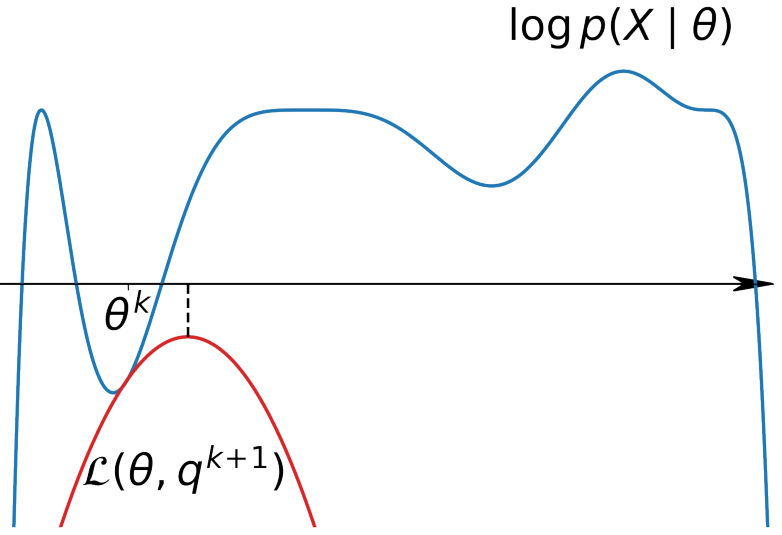
\includegraphics[scale=0.5]{em_1}
\centering
\caption{Optimal choice for $Q$ distribution at E-step in EM makes the lower bound touch the log likelihood function (1-d representation for simplicity)}
\label{fig:em_1} %\ref{fig:em_1}
\end{figure}

Now note that $Q$ is not explicitly known to us, and we define it in a special way so that the Jensen's inequality holds exactly at the equality point when $\theta$ is fixed. This will make the log likelihood exactly equal to the lower bound, and the curves for log likelihood and lower bound would touch at this fixed $\theta$ (fig \ref{fig:em_1}). Thus,
\begin{align*}
    log(p(X|\theta)) &= \sum_{i=1}^{N} \sum_{z_{i}} Q_{i}(z_{i}) log \frac{p(x_{i}, z_{i}|\theta)}{Q_{i}(z_{i})}\\
    0 &= log(p(X|\theta)) - \sum_{i=1}^{N} \sum_{z_{i}} Q_{i}(z_{i}) log \frac{p(x_{i}, z_{i}|\theta)}{Q_{i}(z_{i})}\\
    &= \sum_{i=1}^{N}log(p(x_{i}|\theta)) \times 1 - \sum_{i=1}^{N} \sum_{z_{i}} Q_{i}(z_{i}) log \frac{p(x_{i}, z_{i}|\theta)}{Q_{i}(z_{i})}\\
    &= \sum_{i=1}^{N}log(p(x_{i}|\theta)) \sum_{z_{i}}Q_{i}(z_{i}) - \sum_{i=1}^{N} \sum_{z_{i}} Q_{i}(z_{i}) log \frac{p(x_{i}, z_{i}|\theta)}{Q_{i}(z_{i})}\\
    &= \sum_{i=1}^{N} \sum_{z_{i}}Q_{i}(z_{i}) \bigg( log(p(x_{i}|\theta)) - log \frac{p(x_{i}, z_{i}|\theta)}{Q_{i}(z_{i})} \bigg)\\
    &= \sum_{i=1}^{N} \sum_{z_{i}}Q_{i}(z_{i}) log \frac{p(x_{i}|\theta) Q_{i}(z_{i})}{p(x_{i}, z_{i}|\theta)}\\
    &= \sum_{i=1}^{N} \sum_{z_{i}}Q_{i}(z_{i}) log \frac{p(x_{i}|\theta) Q_{i}(z_{i})}{p(z_{i}|x_{i},\theta)p(x_{i}|\theta)}\\
    &= \sum_{i=1}^{N} \sum_{z_{i}}Q_{i}(z_{i}) log\frac{Q_{i}(z_{i})}{p(z_{i}|x_{i},\theta)}\\
    &= \sum_{i=1}^{N} \KL{Q_{i}(z_{i})}{p(z_{i}|x_{i},\theta)}\\
    \text{For minima,} \quad Q_{i}(z_{i}) &= p(z_{i}|x_{i},\theta) \; \forall \; i = 1,\ldots,N
\end{align*}
since $KL$ divergence $\geq 0$ and the minimum is attained when the two distributions coincide. Thus, E-step is simply setting $Q$ to be the posterior of $z$ given $x$ and $\theta$.\newline

Moving to the M-step, we fix the value of $Q$ and maximize $\mathcal{L}(\theta, Q)$ with respect to $\theta$
\begin{align*}
    \max_{\theta}\mathcal{L}(\theta, Q) &= \max_{\theta} \sum_{i=1}^{N} \sum_{z_{i}} Q_{i}(z_{i}) log \frac{p(x_{i}, z_{i}|\theta)}{Q_{i}(z_{i})}\\
    &= \max_{\theta} \sum_{i=1}^{N} \sum_{z_{i}} Q_{i}(z_{i}) log(p(x_{i}, z_{i}|\theta)) - \sum_{i=1}^{N} \sum_{z_{i}} Q_{i}(z_{i})log(Q_{i}(z_{i}))\\
    &= \max_{\theta} E_{Q}[log(P(X, Z|\theta))]
\end{align*}
i.e., the expectation of the joint distribution of $X$ and latent variables $Z$. Usually this function is concave (we can define in such a way) and local optima are easily achievable.\newline

\subsubsection*{Convergence Guaranties}
The above described EM algorithm leads to an increase in the log likelihood at each step because of the following relations
\begin{alignat*}{2}
    log(P(X|\theta_{k})) &= \mathcal{L}(\theta_{k}, Q_{k+1}) \quad &&\text{equality case in E-step}\\
    \mathcal{L}(\theta_{k}, Q_{k+1}) &\leq \mathcal{L}(\theta_{k+1}, Q_{k+1}) \quad &&\text{M-step to maximize for $\theta$}\\
    \mathcal{L}(\theta_{k+1}, Q_{k+1}) &\leq log(P(X|\theta_{k+1})) \quad &&\text{Jensen's inequality}\\
    \text{or,} \quad log(P(X|\theta_{k})) &\leq log(P(X|\theta_{k+1}))
\end{alignat*}

\subsubsection*{EM Algorithm}
Repeat until convergence
\begin{enumerate}
    \item E-step : set $Q^{(k+1)}_{i}(z_{i}) = p(z_{i}|x_{i}, \theta^{(k)}) (= \argmin_{Q} \sum_{i=1}^{N}\KL{Q_{i}(z_{i})}{p(z_{i}|x_{i}, \theta^{(k)})}$
    \item M-step : $\theta^{(k+1)} = \argmax_{\theta} E_{Q^{(k+1)}}[log(P(X,Z|\theta))]$
\end{enumerate}


%%%%%%%%%%%%%%%%%%%%%%%%%%%%%%%%%%%%%%%%%%%%%%%%%%%%%%%%%%%%%%%%%%%%%%%%%%%
\section{Variational Inference}
The posterior in Bayesian Models with latent variables is quite hard to compute if we do not choose a conjuagte prior for the likelihood function. However, we need to have some approximate version of the posterior in order to make inferences later on. One approach to approximate posterior is to find a distribution $q \in Q$ ($Q$ is a family of distributions) that can minimize the KL divergence
\begin{align*}
    p(z|X) \approx \min_{q \in Q} \KL{q(z)}{p(z|X)}
\end{align*}
where $z$ is the latent variable and $X$ is the data
And we do not need to worry about the normalization constant $Z$ ($p(X)$)
\begin{align*}
    \KL{q(z)}{p(z|X)} &= \int_{z} q(z) log\frac{q(z)}{p(X|z)p(z)/Z}\\
    &= \int_{z} q(z) log\frac{q(z)}{p(X|z)p(z)}  + log(Z)\\
    p(z|X) &\approx \min_{q \in Q} \KL{q(z)}{p(X|z)p(z)} \quad (p(X|z)p(z) = p^{*}(z))
\end{align*}
since $\int_{z} q(z) dz = 1$. We only need to work with likelihood and prior in this case.

\paragraph{E-step in EM} utilizes the variational inference technique. The E-step requires us to calculate the posterior of the latent variables, which can be hard to compute. VI can help us approximate that distribution assuming that we restrict ourselves to a family of distributions.
\begin{align*}
    q(z) = p(z|x, \theta) \approx \min_{q \in Q}KL{q(z)}{p^{*}(z)}
\end{align*}
This is called Variational EM.


%%%%%%%%%%%%%%%%%%%%%%%%%%%%%%%%%%%
\subsection{Mean Field Approximations}
This is a Variational Inference method where we assume the distribution $q$ to be factorized over the latent variables across all dimensions $d$, i.e.,
\begin{align*}
    Q = \{q | q(z) = \prod_{i=1}^{d}q_{i}(z_{i}) \}\\
    q(z) = \argmin_{q \in Q} \KL{\prod_{i=1}^{d}q_{i}(z_{i})}{p^{*}(z)}
\end{align*}
and we minimize the KL divergence using coordinated gradient descent. First find the minima for $q_{1}$ keeping everything else fixed, then $q_{2}$, and so on. We will repeat this loop until convergence.\newline

Since we are minimizing over one component at a time, the functional form of any $q_{k}(z_{k})$ can be derived as follows
\begin{gather*}
    \min_{q_{k}} \KL{\bigg(\prod_{j=1}^{d}q_{j} \bigg)(z_{j})}{p^{*}(z)} = \min_{q_{k}} \int \bigg(\prod_{j=1}^{d}q_{j}(z_{j}) \bigg) log \frac{\prod_{j=1}^{d}q_{j}(z_{j})}{p^{*}(z)} dz \\
    = \min_{q_{k}} \bigg\{ \sum_{i=1}^{d} \int \bigg(\prod_{j=1}^{d} q_{i}(z_{i}) \bigg) log(q_{i}(z_{i})) dz - \int \bigg(\prod_{j=1}^{d}q_{j}(z_{j})\bigg) log(p^{*}(z)) dz \bigg\}\\
    = \min_{q_{k}} \bigg\{ \int \bigg(q_{k}(z_{k})log(q_{k}(z_{k})) \bigg( \int \prod_{j=1, j\neq k}^{d} q_{j}(z_{j}) dz_{\neq j} \bigg) dz_{k} \bigg)\\ + \sum_{i=1, i\neq k}^{d} \int \bigg( q_{i}(z_{i})log(q_{i}(z_{i})) \bigg( \int \prod_{j=1,j \neq i}^{d}q_{j}(z_{j}) dz_{\neq i} \bigg) dz_{i}\bigg) - \int \bigg(\prod_{j=1}^{d}q_{j}(z_{j})\bigg) log(p^{*}(z)) dz \bigg\}\\
    \text{Note that} \quad \int \prod_{j=1}^{d} q_{j}(z_{j}) dz = \int \bigg(\prod_{j=1}^{d} \bigg) q_{j}(z_{j}) dz_{1} dz_{2}\ldots dz_{d} = \prod_{j=1}^{d} \bigg( \int q_{j}(z_{j}) dz_{j}\bigg) = 1\\
    \min_{q_{k}} \bigg\{ \int q_{k}(z_{k})log(q_{k}(z_{k})) dz_{k} + \sum_{i=1, i\neq k}^{d} q_{i}(z_{i})log(q_{i}(z_{i})) dz_{i} \quad \\ \quad  -\int q_{k}(z_{k}) \bigg(\bigg(\prod_{j=1,j\neq k}^{d}q_{j}(z_{j})\bigg) log(p^{*}(z)) dz_{\neq j} \bigg) dz_{k} \bigg\}\\
    = \min_{q_{k}} \bigg\{ \int q_{k}(z_{k}) \bigg[ log(q_{k}(z_{k})) - \bigg(\bigg(\prod_{j=1,j\neq k}^{d}q_{j}(z_{j})\bigg) log(p^{*}(z)) dz_{\neq j} \bigg) \bigg] dz_{k} \bigg \}\\
    \text{because} \quad \sum_{i=1, i\neq k}^{d} q_{i}(z_{i})log(q_{i}(z_{i})) dz_{i} \quad \text{is constant wrt $q_{k}$}
\end{gather*}

We now make three observations
\begin{enumerate}
    \item adding a constant to the minimization equation will still give the same result
    \item $\int q_{k}(z_{k}) dz_{k} = 1$ because $q_{k}$ is a probability distribution
    \item $\int \bigg(\prod_{j=1,j\neq k}^{d}q_{j}(z_{j})\bigg) log(p^{*}(z)) dz_{\neq j} = E_{q_{-k}}[log(p^{*}(z))]$\\
    since $\prod_{j=1,j\neq k}^{d}q_{j}(z_{j})$ is a valid probability distribution. Notice that the expectation integrates over all $z$ except $z_{k}$ and thus is a function of just $z_{k}$. $q_{-k}$ in the expectation just means that we are considering the product $\prod_{j=1,j\neq k}^{d} q_{j}(z_{j})$ as the probability distribution. We convert this expectation to a positive value by taking the exponent, and then get a valid probability distribution as
    \begin{gather*}
        t(z_{k}) = \frac{exp(E_{q_{-k}}[log(p^{*}(z))])}{\int exp(E_{q_{-k}}[log(p^{*}(z))]) dz_{k}}
    \end{gather*}
    The denominator of this expression is a constant which we can introduce in the equation as is without any alteration
\end{enumerate}

Rewriting the minimization equation so far
\begin{gather*}
    \min_{q_{k}} \bigg\{ \int q_{k}(z_{k}) \bigg[ log(q_{k}(z_{k})) - log(exp(E_{q_{-k}}[log(p^{*}(z))])) \bigg] dz_{k} \bigg\} \quad\\ \quad+ \bigg( \int exp(E_{q_{-k}}[log(p^{*}(z))]) dz_{k} \bigg) \int q_{k}(z_{k}) dz_{k} \bigg\}\\
    = \min_{q_{k}} \bigg\{ \int q_{k}(z_{k}) log(q_{k}(z_{k})) - log\frac{exp(E_{q_{-k}}[log(p^{*}(z))])}{\int exp(E_{q_{-k}}[log(p^{*}(z))]) dz_{k}} \bigg\}
    = \min_{q_{k}}\bigg\{\int q_{k}(z_{k}) log\frac{q_{k}(z_{k})}{t(z_{k})}  \bigg\}\\
    \min_{q_{k}} \KL{\bigg(\prod_{j=1}^{d}q_{j} \bigg)(z_{j})}{p^{*}(z)} = \min_{q_{k}} \KL{q_{k}(z_{k})}{t(z_{k})}\\
\end{gather*}
and we know that KL divergence is minimized when the two functions conincide, i.e.
\begin{align*}
    q_{k}(z_{k}) = t(z_{k}) = \frac{exp(E_{q_{-k}}[log(p^{*}(z))])}{\int exp(E_{q_{-k}}[log(p^{*}(z))]) dz_{k}}\\
    \implies \Aboxed{log(q_{k}(z_{k})) = E_{q_{-k}}[log(p^{*}(z))] - constant}
\end{align*}
which is the expectation of the posterior on $z$ over $q$ without the current component being minimized.

\section*{Comparison of Different Inference Methods}
\begin{figure}[h]
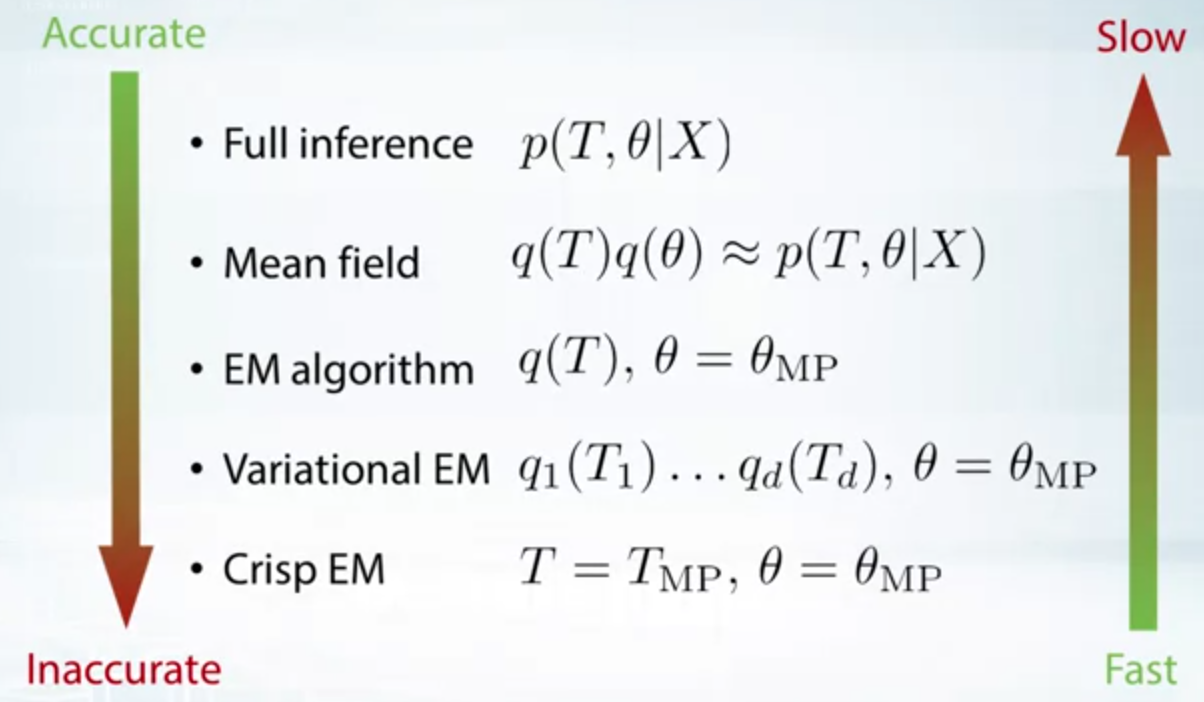
\includegraphics[scale=0.3]{em_2}
\centering
\caption{Comparison of different inference methods in terms of accuracy and inference speed}
\label{fig:em_2} %\ref{fig:em_2}
\end{figure}
\end{document}